\documentclass[8pt, compress]{beamer}

%%% default
%\geometry{paperwidth=128mm,paperheight=96mm}

%\geometry{paperwidth=145mm,paperheight=108.75mm}
\geometry{paperwidth=175mm,paperheight=108.75mm}

%\geometry{paperwidth=150mm,paperheight=112.5mm}
%\geometry{paperwidth=160mm,paperheight=120mm}

\mode<presentation> {
  \usetheme{Warsaw}
 % \usetheme{Boadilla}  
  \setbeamercovered{transparent}
}

% make the navigation bar to disappear
\setbeamertemplate{headline}{}

%\usepackage{ucs}
%\usepackage[czech]{babel}
%\usepackage{czech}
%\usepackage[T1]{fontenc}
%\usepackage[latin2]{inputenc}
\usepackage{array}
\usepackage{times}
\usepackage{palatino}
\usepackage{graphicx}
\usepackage{mathtools}
\usepackage{verbatim}
%\usepackage{RT_woutmeshate}
\usepackage{xmpmulti}

\newcommand{\pdv}[2]{\frac{\partial{#1}}{\partial{#2}}}
\newcommand{\vect}[1]{\boldsymbol{#1}}
\newcommand{\matr}[1]{\mathbf{#1}}
\newcommand{\dI}{\text{d}}
\newcommand{\odv}[2]{\frac{\dI #1}{\dI #2}}
\newcommand{\ddv}[2]{\odv{#1}{#2}}
\newcommand{\mfpe}{\lambda_e}
\newcommand{\mfpei}{\lambda_{ei}}
\newcommand{\Zbar}{Z}
\newcommand{\nue}{\nu_{e}}
\newcommand{\nuei}{\nu_{ei}}
\newcommand{\nuscat}{\nu_{scat}}
\newcommand{\vmag}{v}
\newcommand{\vth}{v_{th}}
\newcommand{\vtwoh}{v_{2 th}}
\newcommand{\vn}{\vect{n}}
\newcommand{\E}{\vect{E}}
\newcommand{\B}{\vect{B}}
\newcommand{\omegaB}{\vect{\omega}_{B}}
\newcommand{\Ez}{E_z}
\newcommand{\qe}{q_e}
\newcommand{\me}{m_e}
\newcommand{\Te}{T_e}
\newcommand{\Ti}{T_i}
\newcommand{\ed}{n_e}
\newcommand{\kB}{k_B}
\newcommand{\fM}{f_M}
\newcommand{\fzero}{f_0}
\newcommand{\vfzero}{\vect{f_0}}
\newcommand{\fone}{{\vect{f_1}}}
\newcommand{\fonez}{f_{1_z}}
\newcommand{\vv}{\vect{v}}
\newcommand{\vvb}{\tilde{\vect{v}}}
\newcommand{\gv}{\nabla_{\vv}}
\newcommand{\gvb}{\nabla_{\vvb}}
\newcommand{\gx}{\nabla_{\vect{x}}}
\newcommand{\ft}{f}
\newcommand{\lnc}{\text{ln}\Lambda}
\newcommand{\Iohm}{\matr{J}_{Ohm}}

\newcommand{\vsp}[1]{\vspace{#1mm}}
\newcommand{\colorimportant}[1]{ {\color{purple} #1} }


%\newenvironment{variableblock}[3]{%
%  \setbeamercolor{block body}{#2}
%  \setbeamercolor{block title}{#3}
%  \begin{block}{#1}}{\end{block}}

% \begin{varblock}[4cm]{Title}
% \end{varblock}
\newenvironment<>{varblock}[2][.9\textwidth]{%
  \setlength{\textwidth}{#1}
  \begin{actionenv}#3%
    \def\insertblocktitle{#2}%
    \par%
    \usebeamertemplate{block begin}}
  {\par%
    \usebeamertemplate{block end}%
  \end{actionenv}}

\newcommand\myheading[1]{%
  \par\bigskip
  {\large\bfseries#1}\par\smallskip}

%%%%%%%%%%%%%%%%%%%%%%%%%%%%%%%%%%%%%%%%%%%%%%%%%%%%
%%%                pcolumn                       %%%
%%%%%%%%%%%%%%%%%%%%%%%%%%%%%%%%%%%%%%%%%%%%%%%%%%%%

\newenvironment{pcolumn}[1]{
  \begin{minipage}{#1\textwidth}
  \begin{center}
}{
  \end{center}
  \end{minipage}
}
  
%%%%%%%%%%%%%%%%%%%%%%%%%%%%%%%%%%%%%%%%%%%%%%%%%%%%
%%%                mycaptionfig                     %%%
%%%%%%%%%%%%%%%%%%%%%%%%%%%%%%%%%%%%%%%%%%%%%%%%%%%%
% \mycaptionfig - replacement for \caption
% necessary, since in multicol-environment \figure and
% therefore \caption won't work

%\newcounter{figure}
\setcounter{figure}{1}
\newcommand{\mycaptionfig}[1]{
  %\vspace{0.5cm}
  \vspace{0.05cm}
  \begin{quote}
    {{\sc Fig} \arabic{figure}: #1}
  \end{quote}
  %\vspace{1.0cm}
  \vspace{0.2cm}
  \stepcounter{figure}
}
  
\setcounter{table}{1}
\newcommand{\mycaptiontable}[1]{
  %\vspace{0.5cm}
  \vspace{0.05cm}
  \begin{quote}
    {{\sc Table} \arabic{table}: #1}
  \end{quote}
  %\vspace{1.0cm}
  \vspace{0.2cm}
  \stepcounter{table}
}
  
\useinnertheme{rectangles}
%\useoutertheme{infolines} 

\title[AWBS electrons kinetic modeling with nonlocal Ohm’s law\\ in plasmas relevant to inertial confinement fusion]{AWBS kinetic modeling of electrons with nonlocal Ohm’s law\\ in plasmas relevant to inertial confinement fusion
%\\
%\textit{Serious Numerics for Serious Physics}
}
\author[Milan~Holec]{{\large Milan~Holec, Dario Del Sorbo}}
%\institute[US JAK]{
%         {\large CELIA, University of Bordeaux,\\ 
%		 33405 Talence, France
%		 \\ 
%		 ({\tt milan.holec@u-bordeaux.fr})
%		 }
%         }

\date{
	\begin{figure}
    \begin{center}
	\begin{tabular}{ccc} 
	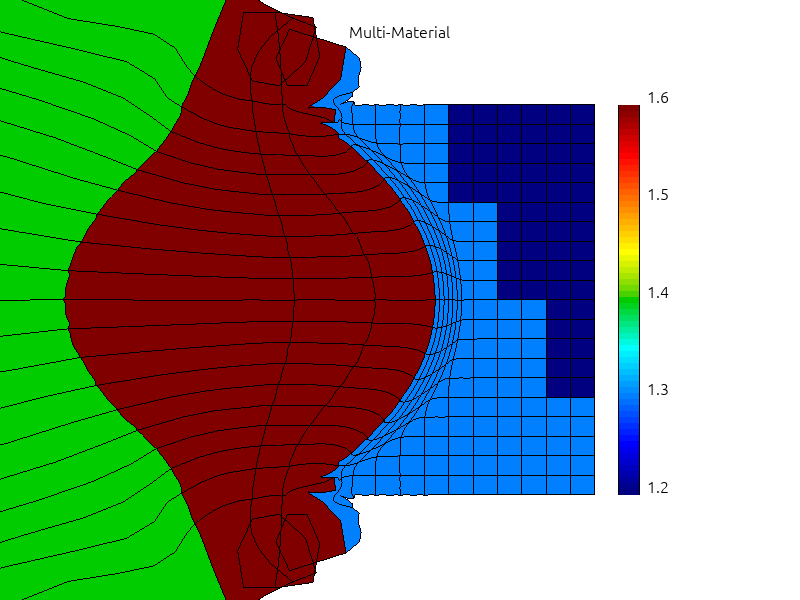
\includegraphics[width=0.3\textwidth]{../figures/material_77.png}
	&
	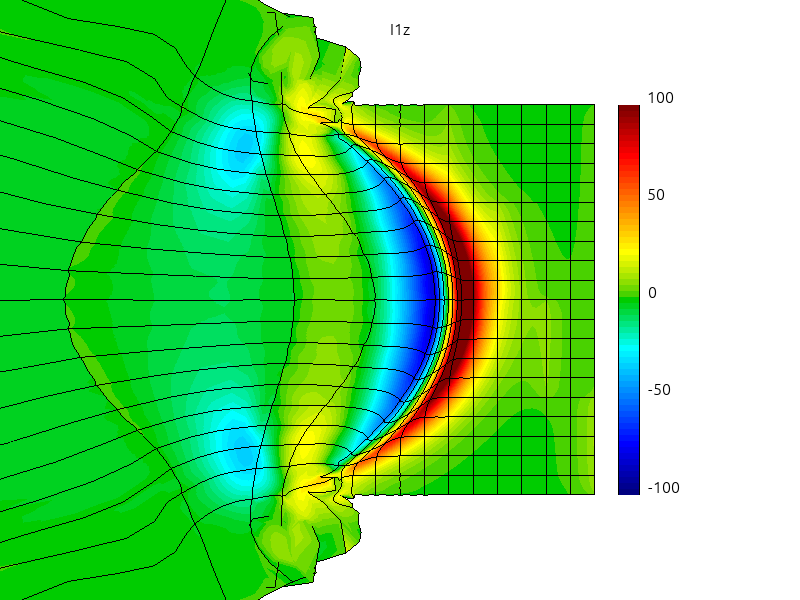
\includegraphics[width=0.3\textwidth]{../figures/nonlocalI1z_77.png}
	&
	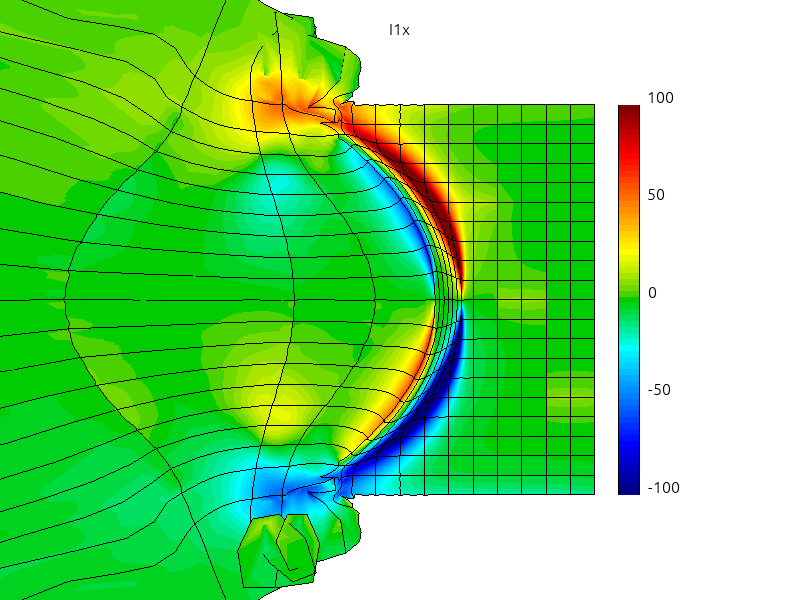
\includegraphics[width=0.3\textwidth]{../figures/nonlocalI1x_77.png}
	\end{tabular}
	\end{center}
	\end{figure}
	\begin{tabular}{c}	
	LLNL - ClubMED,\\
	Livermore, CA,\\
	Jan 7, 2019 
	\end{tabular}
}
%\date{COST Working Group Meeting\\
%Advanced X-ray spatial and temporal metrology\\
%July 9-10, 2015, Madrid}      

\defbeamertemplate*{footline}{miniframes theme}%{shadow theme}
{%
  \leavevmode%
  \hbox{\begin{beamercolorbox}[wd=.5\paperwidth,ht=2.5ex,dp=1.125ex,leftskip=.3cm plus1fil,rightskip=.3cm]{author in head/foot}%
    \usebeamerfont{author in head/foot}\insertframenumber\,/\,\inserttotalframenumber\hfill\insertshortauthor
  \end{beamercolorbox}%
  \begin{beamercolorbox}[wd=.5\paperwidth,ht=2.5ex,dp=1.125ex,leftskip=.3cm,rightskip=.3cm plus1fil]{title in head/foot}% 
    \usebeamerfont{title in head/foot}\insertshorttitle% 
  \end{beamercolorbox}}%
  \vskip0pt%
}      
      
\begin{document}
\begin{frame}
 \titlepage
\end{frame}

%\begin{frame}
%  \tableofcontents
%\end{frame}

\section{Introduction to Nonlocal Magneto-Hydrodynamic model (Nonlocal-MHD)}

%\subsection{Nonlocal electron transport}
\newcommand{\edf}{\colorimportant{f}}
\begin{frame}
\begin{center}
{\huge Hydrodynamic model of plasma}
\begin{block}{Fokker-Planck/Boltzmann transport equation}
\begin{equation}
  \frac{\partial \edf}{\partial t} + 
  \vect{v}\cdot\nabla_x \edf + \frac{q_e}{m_e}\left(\vect{E}
  +\frac{\vect{v}}{c}\times\vect{B}\right)\cdot
  \nabla_{\vect{v}} \edf 
  = 
  \sigma \nabla_{\vect{v}}\cdot\int 
  \frac{|\vect{v}-\vect{v}'|^2\matr{I} - (\vect{v}-\vect{v}')\otimes 
  \vect{v}-\vect{v}')}{|\vect{v}-\vect{v}'|^3}
  \big(\nabla_{\vect{v}} \edf(\vect{v}) f(\vect{v}') - 
  \edf(\vect{v}) \nabla_{\vect{v}} f(\vect{v}')\big) \dI \vect{v}'
  \label{eq:FP}
  %C(\edf, \edf)
  %\nonumber
\end{equation}
\end{block}
\begin{block}{Fluid equations in Lagrangian frame (velocity space moments of \eqref{eq:FP})}
\begin{eqnarray}
	\frac{\dI \rho}{\dI t} &=& - \rho \nabla\cdot\vect{U}%\, ,
	\label{lagrange_ei_mass_equation} \nonumber\\
	\rho \frac{\dI \vect{U}}{\dI t} 
    &=& \nabla\cdot\matr{\sigma} + \vect{j}\times\B%\, ,
	\label{lagrange_ei_momentum_equation} \nonumber\\
	\rho\frac{\dI \varepsilon}{\dI t} &=& 
	\matr{\sigma}:\nabla\vect{U}
	- \nabla\cdot\vect{q}_e%\, ,
	\label{lagrange_i_energy_equation} \nonumber
\end{eqnarray}
\end{block}
\begin{block}{Microscopic closure}
\begin{eqnarray}
	\matr{\sigma} &=& -\rho
	\int (\vect{v}-\vect{U})\otimes
	(\vect{v}-\vect{U})\, \edf\, \dI \vect{v}^3 \approx -\matr{I} p 
	+ \tilde{\matr{\sigma}}(\nabla \vect{U})
	\label{stress_tensor}\nonumber\\
	\vect{q}_e &=& \frac{\me}{2} 
	\int |\vect{v} - \vect{U}|^2
	(\vect{v}-\vect{U})\, \edf\, \dI \vect{v}^3 \approx 
	\frac{\me}{2} 
	\int_{4\pi}\vect{n}\int_0^\infty 
	|\vect{v}|^5 \edf\, \dI |\vect{v}|\, \dI \vect{n}
	\approx -\kappa(T^{2.5})\nabla T 
	\label{heat_flux_vector} \nonumber
    \\
    \vect{j} &=& \qe 
	\int(\vect{v}-\vect{U})\, \edf\, \dI \vect{v}^3
    \nonumber
    %\\
	%\vect{q}_R &=& \int_{4\pi} \vect{n} \int_\nu I^{~p}_\nu\, \dI \nu\, 
	%\dI \vect{n} \approx - \int_\nu \frac{c}{\chi_\nu} \nabla ( f_\nu E_\nu) 
    %\, \dI \nu
	%\label{radiation_flux_vector} \nonumber
\end{eqnarray}
\end{block}
\end{center}
\end{frame}

\begin{comment} % SH
\begin{frame}
\begin{center}
Spitzer-Harm electron diffusion
\begin{block}{BGK collision operator}
\begin{eqnarray}
  C_{ei}(f^e, f^i)&\stackrel{m_e/m_i}{\approx}& 
  \sigma \nabla_v\cdot\left(\frac{1}{v}
  \left( \matr{I} - \frac{\vect{v}\otimes\vect{v}}{v^2}\right)\cdot\nabla_v 
  f^e\right)
  \nonumber\\
  &\stackrel{\text{spher}}{\approx}& \frac{\sigma}{v^3}
  \frac{1}{\sin(\phi)}\left[\frac{\partial}{\partial \phi}
  \left(\sin(\phi)\frac{\partial f^e}{\partial \phi}\right) 
  + \frac{1}{\sin(\phi)}\frac{\partial^2f^e}{\partial \theta^2}\right] 
  \nonumber \\
  &\stackrel{f^0 + f^1\cos(\phi)}{\approx}& 
  - \frac{2 \sigma}{v^3} f^e_1\cos(\phi) = 
  2 \nu_{ei} \left(f^e_0  - f^e\right) \nonumber
\end{eqnarray} 
\end{block}
Then, the~electron distribution function can be governed by the~BGK Boltzmann transport equation
\begin{equation}
  %\frac{1}{|\vect{v}|}\frac{\partial f^e}{\partial t} + 
  \vect{n}\cdot\nabla_x f^e + \frac{q_e}{m_e |\vect{v}|}\vect{E}\cdot
  \nabla_{\vect{v}} f^e 
  = 
  \frac{2 (f_{MB}(|\vect{v}|, T_e) - f^e)}{\lambda_{ei}}\, , 
  \nonumber
\end{equation}
where $f_{MB}$ is the~Maxwell-Boltzmann equilibrium distribution and 
$\lambda_{ei}$ the~electron mean free path when scattered on ions.
%\begin{eqnarray}
%  \frac{1}{\bar{v}}\frac{\partial I^e}{\partial t} + \vect{n}\cdot\nabla I^e 
%  &=& 
%  \frac{\sigma^e T_e - I^e}{\lambda^e}\, , 
%  \nonumber
%  \\
%  \vect{q}_e &=& \int_{4\pi}\vect{n}\, I^e\, \dI\vect{n}\,  ,
%  \nonumber
%\end{eqnarray}
\begin{block}{Chapman-Enskog approximation in small parameter $\lambda_{ei}$}
\begin{equation}
 f^e = f_0 + \lambda_{ei} f_1 + O({\lambda_{ei}}^2) \approx 
 f_{MB}(|\vect{v}|, T_e)
 - f_{MB}(|\vect{v}|, T_e) g(\bar{Z})
   \left(\frac{|\vect{v}|^2}{2 v_{T_e}^2} - 4\right)
    \vect{n}\cdot\frac{\lambda_{ei}\nabla T_e}{T_e}\nonumber
\end{equation}
\begin{equation}
  \rightarrow \vect{q}_{SH} = \kappa_{SH}\, T_e^{\frac{5}{2}}\, \nabla T_e
  \nonumber 
\end{equation}
%$I \approx \sigma T_e - \lambda \vect{n}\cdot
%  \nabla \left(\sigma T_e\right) + O(\lambda^2)$ 
%$\rightarrow \vect{q} \approx - \lambda \sigma \nabla T_e$ 
\end{block}
\begin{equation}
	\frac{\lambda_{ei} f_1}{f_0} = 0.25
	\left(\frac{|\vect{v}|^2}{2 v_{T_e}^2} - 4\right)
	\vect{n}\cdot\frac{\lambda_{ei}(|\vect{v}|^4)\nabla T_e}{T_e} < 0.1
	\quad\longrightarrow\quad \text{Kn}^e = \frac{\lambda_{ei}\nabla T_e}{T_e} 
	< 7.5\times10^{-4}
	\nonumber \label{SH_limit}
\end{equation}
\end{center}
\end{frame}
\end{comment} % SH

\begin{frame}
\begin{center}
{\huge Local diffusive transport regime}
\begin{block}{Collision operators}
    \begin{eqnarray}
        C_{FP} &=& \Gamma_{ee}\int \gv\gv(\vv - \vvb) \cdot \left(
        \ft\, \gvb \ft - \ft\, \gv \ft \right)\, \dI\vvb
        + \frac{\nuei}{2} 
        \pdv{}{\mu}\left((1 - \mu^2)\pdv{f}{\mu}\right)
        \\
        C_{BGK} &=& \nue(\fM - \ft)
        + \frac{\Zbar + 4.2}{\Zbar + 0.24}\frac{\nuei}{2} 
        \pdv{}{\mu}\left((1 - \mu^2)\pdv{f}{\mu}\right)
        \\
        C_{FP0} &=& 
        v \nue\frac{\partial}{\partial v}
        \left[C(\fzero)\fzero
        + D(\fzero)\frac{\partial \fzero}{\partial v}\right]
        + \frac{\Zbar + 4.2}{\Zbar + 0.24}\frac{\nuei}{2} 
        \pdv{}{\mu}\left((1 - \mu^2)\pdv{f}{\mu}\right)
        \\
        C_{AWBS} &=& \vmag \frac{\nue}{2}
        \pdv{}{\vmag}\left(\ft - \fM\right)
        + \frac{\nuei + \frac{\nue}{2}}{2} 
        \pdv{}{\mu}\left((1 - \mu^2)\pdv{f}{\mu}\right)       
    \end{eqnarray}
\end{block}

\begin{tabular}{c}
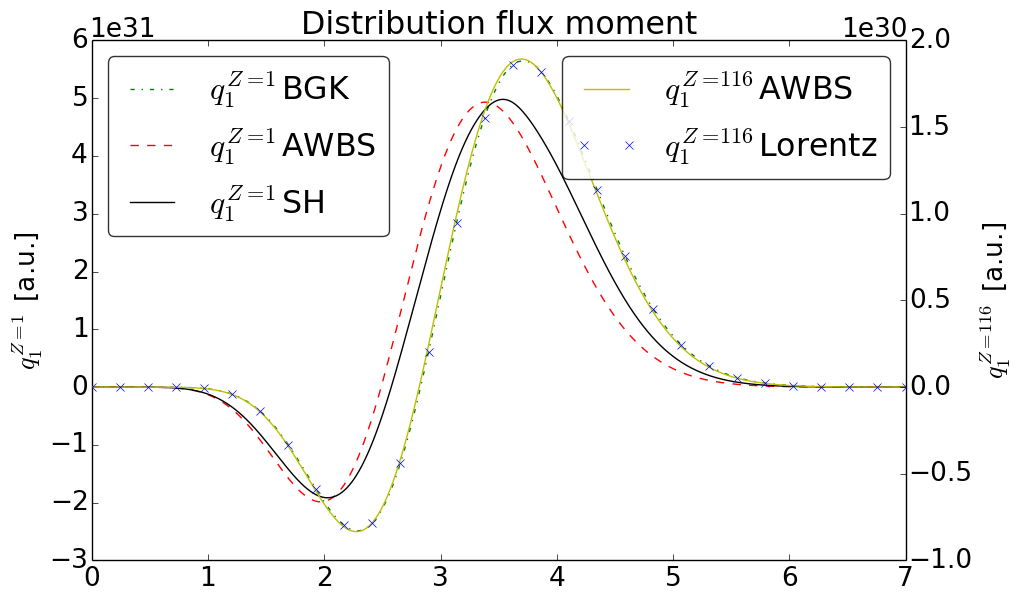
\includegraphics[width=0.5\textwidth]{../figures/q1s.png}
\end{tabular}
\begin{tabular}{c|ccccc}
    %\hline
    %$\Zbar$ & $1$ & $2$ & $4$ & $16$ & $\infty$ \\\\
    & $\,Z=1\,$ & $\,Z=2\,$ & $\,Z=4\,$ & $\,Z=16\,$ & $\,Z=116\,$ 
	\\
    \hline
    $\bar{\Delta}\mathbf{q}_{AWBS}$ & 0.057 & 0.004 & 0.037 & 0.021 & 0.004 \\
    %\hline\\
    %$\phi(Z)$ & -0.037 & -0.003 & 0.04 & 0.058 & 0.065 \\\\ 
    %\hline
\end{tabular}

%Z-dependence of electron distribution function (heat flux moment) by AWBS, Spitzer and Harm, and VFP operator $C^{FP}_{ee}(\fzero) = 
%v \nue\frac{\partial}{\partial v}
%\left[C(\fzero)\fzero+D(\fzero)\frac{\partial \fzero}{\partial v}\right]$. 
AWBS provides excellent results for any Z.

\end{center}
\end{frame}

\newcommand{\fs}{0.33}
\begin{frame}
\begin{center}
{\huge Nonlocal electron transport regime - PIC/VFP0/AWBS}

\begin{tabular}{ccc}
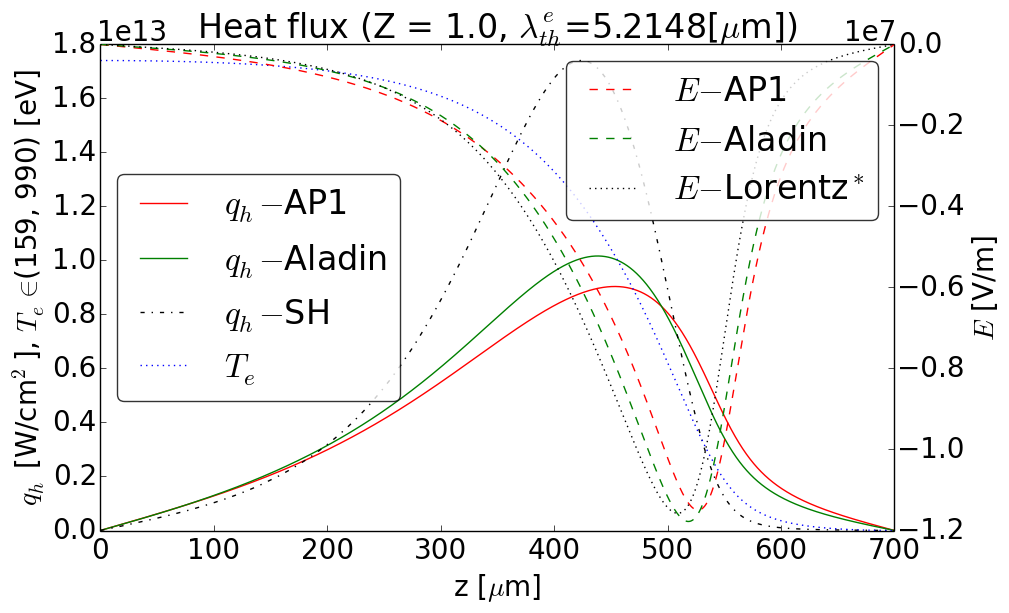
\includegraphics[width=\fs\textwidth]{../figures/C7_Aladin_case5_heatflux.png}
&
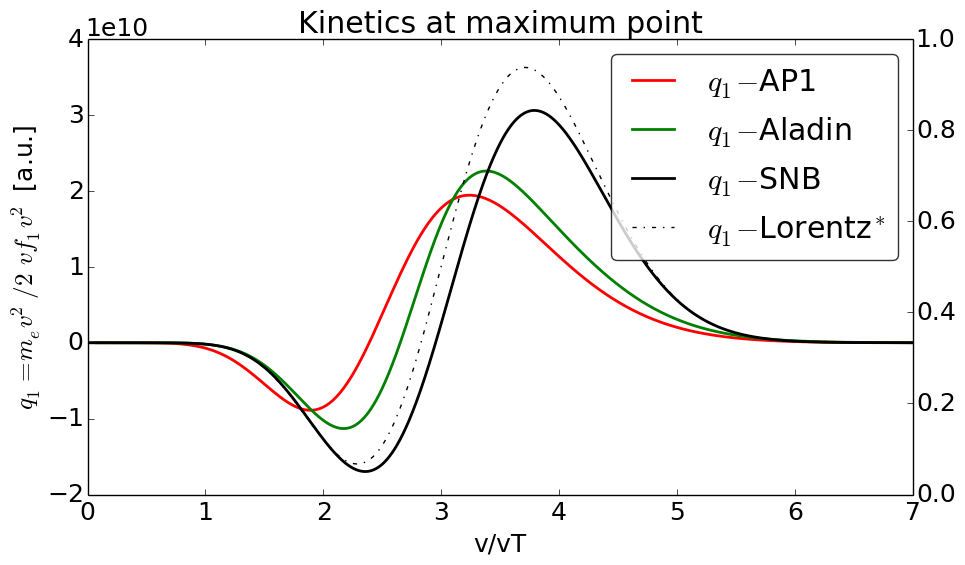
\includegraphics[width=\fs\textwidth]{../figures/C7_Aladin_case5_kinetics.png}
&
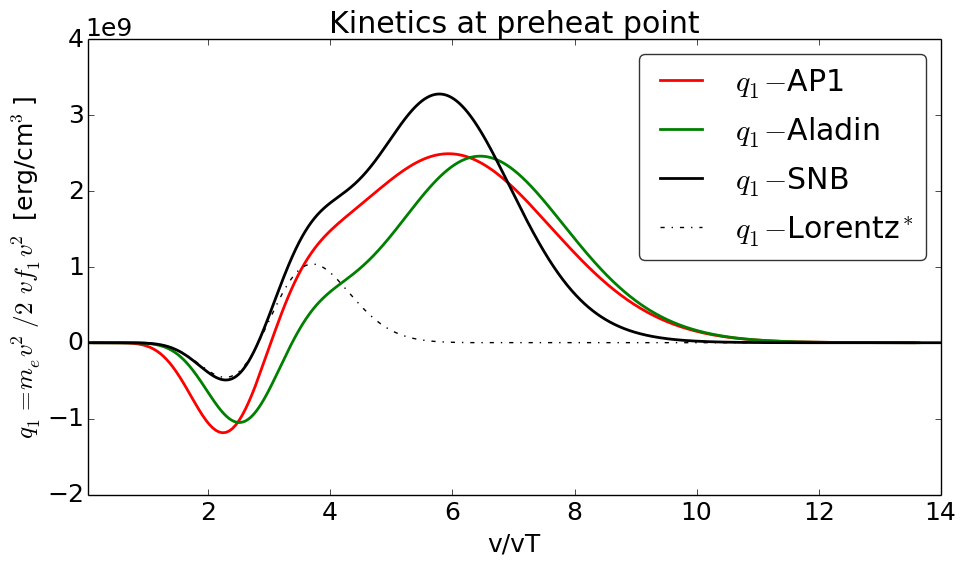
\includegraphics[width=\fs\textwidth]{../figures/C7_Aladin_case5_nonlocal_kinetics.png}
\\
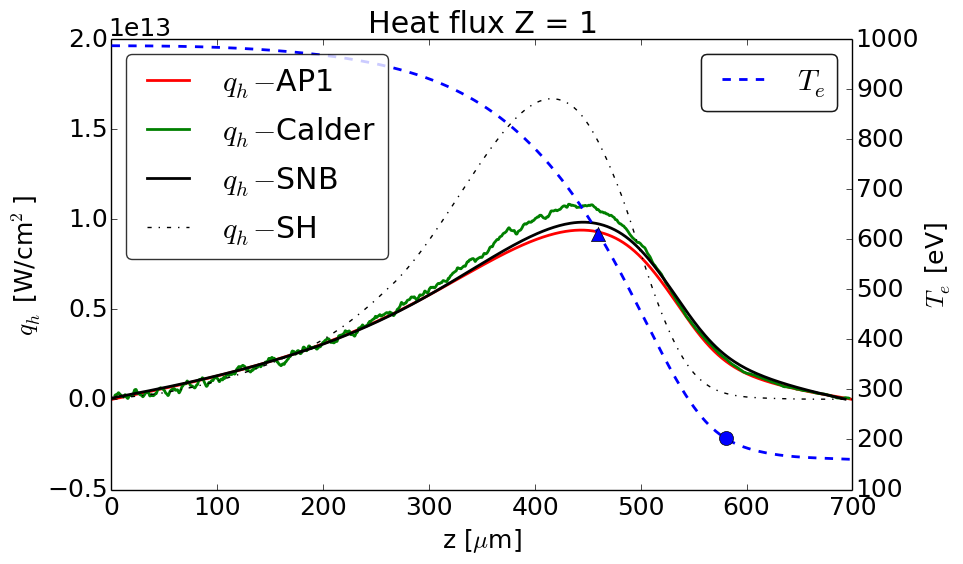
\includegraphics[width=\fs\textwidth]{../figures/C7_Calder_case5_heatflux.png}
&
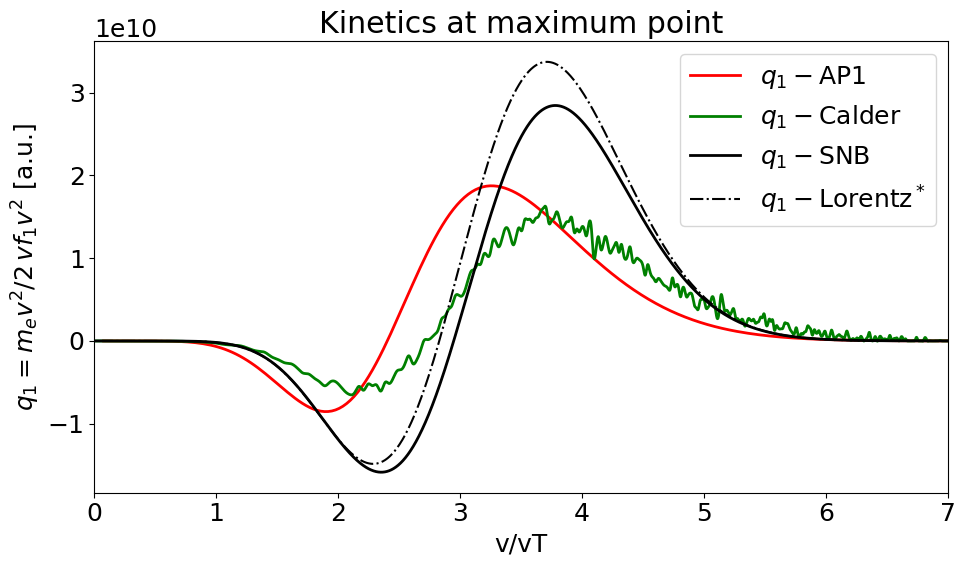
\includegraphics[width=\fs\textwidth]{../figures/C7_Calder_case5_kinetics.png}
&
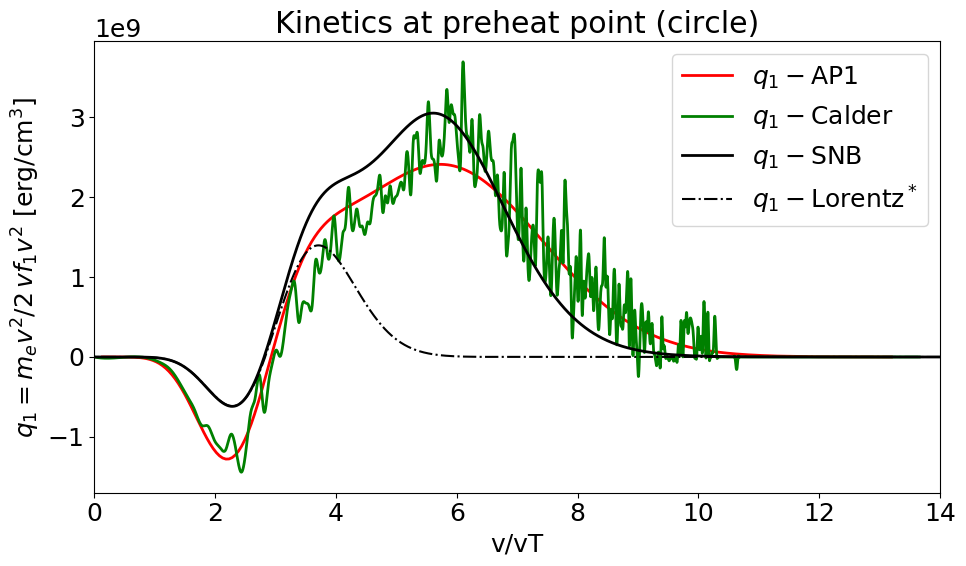
\includegraphics[width=\fs\textwidth]{../figures/C7_Calder_case5_nonlocal_kinetics.png}
\end{tabular}
\end{center}
\end{frame}

\begin{frame}
\begin{center}
{\huge Electron velocity limit - friction vs. $\vect{E}$ stopping}
\begin{equation}
  \pdv{\ft}{t} + \vv\cdot\nabla \ft + 
  \frac{\qe}{\me}\left(\E + \frac{\vv}{c}\vect{\times}\B\right)
  \cdot\pdv{\ft}{\Omega} =  
  \left(\vmag \frac{\nue}{2} -  \frac{\qe}{\me}~\vv\cdot\E \right)
  \pdv{\ft}{\vmag} - \vmag \frac{\nue}{2}\pdv{\fM}{\vmag}
  + \frac{\nuei +\frac{\nue}{2}}{2} \frac{\partial^2\ft}{\partial\Omega^2},
  \nonumber\label{eq:kinetic_equation}
\end{equation}
\begin{tabular}{c|ccccc}
    \hline\hline\\
    %Kn$^e$ & $10^{-4}$ & $10^{-3}$ & $10^{-2}$ & $10^{-1}$ & $1$ \\\\
    Kn$^e$ & $\,\,10^{-4}\,\,$ & $\,\,10^{-3}\,\,$ & $\,\,10^{-2}\,\,$ & $\,\,10^{-1}\,\,$ & $\,\,1\,\,$ \\\\
    \hline\\
    $v_{lim} / v_{th}$ & 70.8 & 22.4 & 7.3 & 3.1 & 1.8\\\\
    \hline\hline
\end{tabular} 

\begin{tabular}{c}
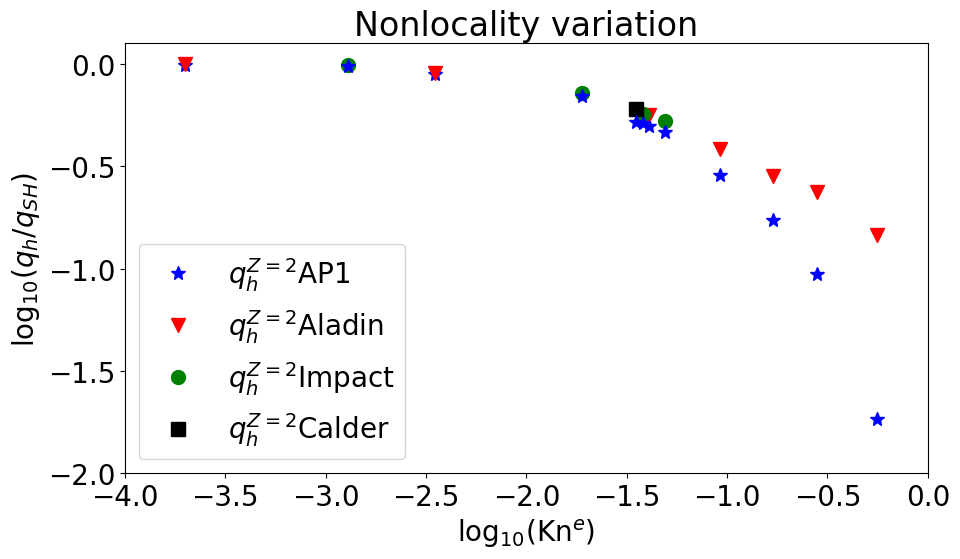
\includegraphics[width=0.5\textwidth]{../figures/Kn_results.png}
\end{tabular}

$\vect{E}$ stopping overtakes collisions for Kn$>0.1$.

\end{center}
\end{frame}

\begin{frame}
\begin{center}
%{\huge NIF relevant conditions}

{\large NIF hohlraum - plasma profiles provided by HYDRA}

\begin{tabular}{c}
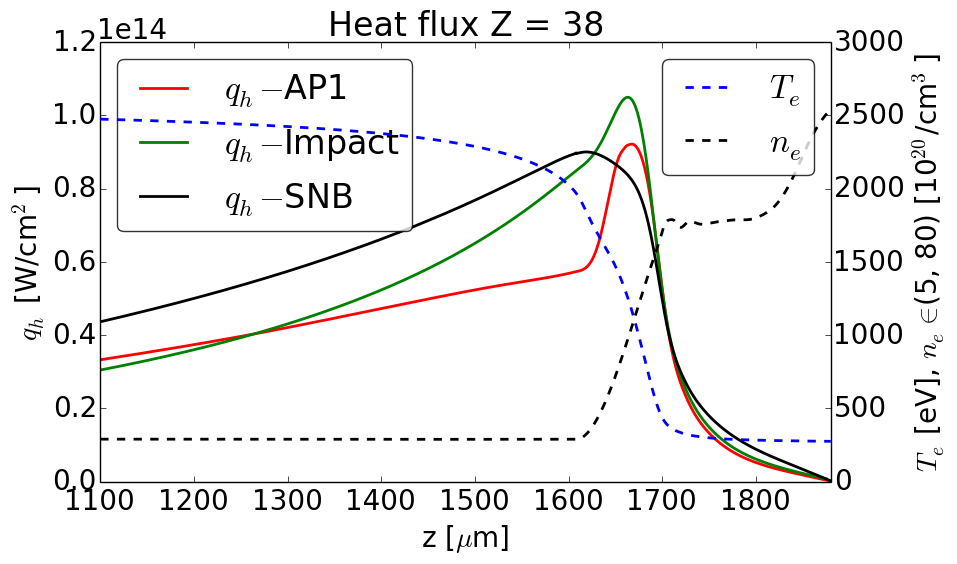
\includegraphics[width=0.5\textwidth]{../figures/C7_GdHohlraum_heatflux.png}
\end{tabular}

{\large SNB approach}
\begin{equation}
  \tilde{\ft} = 
  \fM + \delta\fzero 
  + \Omega\cdot\left(\fone_M + \delta\fone\right) . 
  \nonumber\label{eq:SNB_approximation}
\end{equation}
\begin{equation}
    \fone_M = -\frac{\Zbar + 0.24}{\Zbar + 4.2}\mfpei\fM\left( \frac{\nabla\ed}{\ed} 
  + \left( \frac{\vmag^2}{2\vth^2} - \frac{3}{2}\right)
  \frac{\nabla\Te}{\Te} - \frac{\qe\E_L}{\me\vth^2}\right) ,
  \qquad\E_L = \frac{\me\vth^2}{\qe}\left(\frac{\nabla\ed}{\ed} 
  + \frac{5}{2}\frac{\nabla\Te}{\Te} \right)
  \nonumber
\end{equation}

\end{center}
\end{frame}

\begin{frame}
\begin{center}
{\Huge Nonlocal Ohm's law}

We found that the~quality of the~electric field evaluation is essential for 
a~correct plasma modeling 
\begin{block}{Nonlocal current in plasma}
\begin{equation}
  \vect{j}(f, \vect{E}) = e \int v \fone v^2~\dI v = 
  e \int v \frac{\nuei^2 \vect{E}^* 
  + \omegaB~\omegaB\cdot\vect{E}^* + \nuei~\omegaB \times \vect{E}^*}
  {\nuei (\omegaB^2 + \nuei^2)} v^2~\dI v ,
  \label{eq:NonlocalOhm}
\end{equation}
\end{block}
where $\vect{E}^* = \vmag\frac{\nue}{2}\pdv{\fone}{\vmag} - \vmag\nabla\fzero 
 - \frac{\qe}{\me}\E\pdv{\fzero}{\vmag}$ 
is an effective electric field in plasma. 
A~comparison to the \textit{Generalized Ohm's law} shows a~correct local 
behavior of \eqref{eq:NonlocalOhm}, especially that 
$\nabla\times \nabla \fzero \sim \nabla\times \frac{\nabla p_e}{\ed} \sim \nabla n_e \times \nabla T_e$

\begin{block}{Generalized Ohm's law vs. nonlocal Ohm's law}
\begin{eqnarray} 
  \vect{E} &=&  
  \left(\vect{R}_T -\nabla p_e\right)\quad + ~~~~~\quad\qquad 
  \frac{\vect{j}}{\sigma}\qquad\quad ~~~~+
  \qquad \vect{j}\times\vect{B} ,
  \nonumber \\
  \vect{E} \vmag \frac{\qe}{\me}\pdv{\fzero}{\vmag} 
  &=& 
  ~~~~\vmag^2 \nabla\fzero ~~~~~~~~~ 
  +~~~  \vmag^2 \frac{\nue}{2}\pdv{\fone}{\vmag} - \vmag \nuei\fone 
  ~~~+~~~ v \fone\times\frac{\qe}{\me c}\vect{B}.
  %\vect{E} \int v \pdv{\fzero}{v} v^2\, \dI v 
  %&=& 
  %\int v^2 \nabla \fzero v^2\, \dI v~~~ +~~  \int v \nuei\fone v^2\, \dI v 
  %~~~+~~ \int v \fone\times\vect{B} v^2\, \dI v .
  \nonumber
\end{eqnarray}
\end{block}

\end{center}
\end{frame}

\begin{frame}
\begin{center}
{\huge Nonlocal-MHD}  

\begin{eqnarray}
  \text{HYDRODYNAMICS} && \nonumber \\
  && \nonumber \\
  \frac{\dI \rho}{\dI t} &=& - \rho\nabla\cdot\vect{u} , 
  \nonumber\\ 
  \rho\, \frac{\dI \vect{u}}{\dI t} &=& - \nabla (p_i + p_e) 
  + \vect{j}(f, \vect{E}) \times \vect{B}, 
  \nonumber\\   
  \rho \left(\frac{\partial \varepsilon_i}{\partial T_i}\frac{\dI T_i}{\dI t} 
  +\frac{\partial \varepsilon_i}{\partial \rho}\frac{\dI \rho}{\dI t}\right)
  &=& 
  - p_i\nabla\cdot\vect{u} - G(T_i - T_e) , 
  \nonumber\\
  \rho \left(\frac{\partial \varepsilon_e}{\partial T_e}\frac{\dI T_e}{\dI t}
  +\frac{\partial \varepsilon_e}{\partial \rho}\frac{\dI \rho}{\dI t}\right)
  %+ \frac{\dI \epsilon_R}{\dI t} 
  &=& 
  - p_e \nabla\cdot\vect{u} - \nabla\cdot\vect{q}_e(f) + 
  G(T_i - T_e) + Q_{\text{IB}}(\vect{E}_L) , 
  \nonumber \\
  && \nonumber \\
  && \nonumber \\
  \text{MAXWELL EQUATIONS} && \nonumber \\
  && \nonumber \\
  \nabla\times\vect{E} &=& -\frac{1}{c}\frac{\dI \vect{B}}{\dI t} ,
  %\quad\qquad (\text{life of magnetic field}~\vect{B}~\text{in the fluid frame})
  \nonumber \\
  \nabla\times\vect{B} &=& \frac{4\pi}{c}
  \vect{j}(f, \vect{E}) ,%\quad~~~ (\vect{j} \text{ depends on }f\text{ and }\vect{E}\text{ from the nonlocal model}) 
  \nonumber \\
  && \nonumber \\
  %&& \nonumber \\
  \text{AWBS KINETICS OF ELECTRONS} && \nonumber \\
  && \nonumber \\
  \pdv{f}{t} + \vect{v}\cdot\nabla f +
  \left( \vect{E} + \vect{v}\times\vect{B}\right)\cdot\nabla_{\vect{v}} f
  &=& 
  v \frac{\nue}{2} \frac{\partial }{\partial v}\left(f - f_{MB}(T_e)\right)
  + \frac{\nuei + \frac{\nue}{2}}{2} \frac{\partial^2 f}{\partial \Omega^2} .
  \nonumber \label{eq:AWBS}
\end{eqnarray}

\end{center}
\end{frame}

\begin{comment} % NonlocalRadHydro
\begin{frame}
\begin{center}
{\large Thermal Radiative Transfer}
\begin{block}{Radiation transport equation}
The~radiation intensity $I_\nu(\vect{x}, \vect{n})$ representing photons of frequency $\nu$ obeys the~equation
\begin{equation}
  \vect{n}\cdot\nabla I_\nu = \eta_\nu - \chi_\nu I_\nu , 
  \nonumber \label{eq:RT}
\end{equation}
where \textit{emmisivity} $\eta_\nu(\rho, T)$ and absorptivity 
$\chi_\nu(\rho, T)$ are considered to be isotropic.
\end{block}
\begin{eqnarray}
  \nabla \cdot \vect{q}_\nu &=& 4\pi\eta_\nu - \chi_\nu E_\nu  \nonumber \\
  \nabla \cdot \matr{P}_\nu &=& -\frac{\chi_\nu}{c}\vect{q}_\nu \nonumber
\end{eqnarray}
\begin{block}{Radiation diffusion}
In the~case of low anisotropy pressure tensor can be approximated as
$\matr{P}_\nu = \matr{I} f_\nu E_\nu$ and the~radiation field can be modeled by
\begin{equation}
  \nabla \cdot \left( \frac{c}{\chi_\nu} \nabla ( f_\nu E_\nu) \right) = 
  \chi_\nu E_\nu - 4\pi\eta_\nu , 
  \nonumber
\end{equation}
where the~lowest anisotropy approximation 
$\tilde{I}_\nu(\vect{x}, \vect{n}) = I^0_\nu(\vect{x}) 
+ \vect{n}\cdot\vect{I}^1_\nu(\vect{x})$ 
corresponds to the~\textit{variable Eddington factor} 
$f_\nu = \frac{1}{3}$.
\end{block}
\end{center}
\let\thefootnote\relax\footnote{D. Mihalas and B. Mihalas, Foundations of Radiation Hydrodynamics 
(Oxford University Press, New York, 1985).}
\end{frame}

\subsection{Nonlocal Magneto-Hydrodynamic model}
\begin{frame}
\begin{center}
{\large Nonlocal Magneto-Hydrodynamic model}
%\myheading{Radiative Fluid Model of Laser Plasma}
%Conservation of mass $\rho$, momentum $\rho \vect{u}$, 
%and energy $\varepsilon_e+\varepsilon_i+\epsilon_R$ of radiation field 
%and plasma fluid, 
%where the inverse-bremsstrahlung deposition of laser electric
%field $\vect{E}_L$ heats the target, read 
\begin{eqnarray}
 \frac{\dI \rho}{\dI t} &=& - \rho\nabla\cdot\vect{u}\, , 
 \nonumber\\ 
 \rho\, \frac{\dI \vect{u}}{\dI t} &=& - \nabla (p_i + p_e + p_{\vect{B}}) \, , 
 \nonumber\\   
 \rho \left(\frac{\partial \varepsilon_i}{\partial T_i}\frac{\dI T_i}{\dI t} 
 +\frac{\partial \varepsilon_i}{\partial \rho}\frac{\dI \rho}{\dI t}\right)
 &=& 
 - p_i\nabla\cdot\vect{u} - G(T_i - T_e)\, , 
 \nonumber\\
 \rho \left(\frac{\partial \varepsilon_e}{\partial T_e}\frac{\dI T_e}{\dI t}
 +\frac{\partial \varepsilon_e}{\partial \rho}\frac{\dI \rho}{\dI t}\right)
  %+ \frac{\dI \epsilon_R}{\dI t} 
  &=& 
 - p_e \nabla\cdot\vect{u} - \nabla\cdot\left(\vect{q}_e+\vect{q}_R \right) + 
 G(T_i - T_e) + Q_{\text{IB}}(\vect{E}_L)\, , 
 \nonumber
\end{eqnarray}
the quantities $\frac{\partial \varepsilon}{\partial \rho} =
\frac{\partial f}{\partial \rho}
- T \frac{\partial^2 f}{\partial \rho \partial T}$, 
$\frac{\partial \varepsilon}{\partial T} = 
-T \frac{\partial^2 f}{\partial T^2}$, 
$p = \rho^2 \frac{\partial f}{\partial \rho}$, 
$G = \rho\frac{\partial \varepsilon_e}{\partial T_e} \nu_{ei}$ 
provides our HerEOS equation of state.
\footnote{M. Zeman, M. Holec, P. Vachal, "HerEOS: a Framework for Consistent Treatment of the Equation of State in ALE Hydrodynamics",\\ 
\textit{Comp. Math. Appl.}, submitted (2017).}
%and depend on ion and electron free energies $f_i(\rho, T_i)$, 
%$f_e(\rho, T_e)$ locally. 

\begin{tabular}{c|c}
\hline \\

\begin{pcolumn}{0.42}
Nonlocal transport of photon intensity 
$I^p=\int_\nu f^p\, \frac{h^4\nu^3}{c^2}\, \dI\nu$
\begin{equation}
  %\frac{1}{c}\frac{\partial I^p}{\partial t} + 
  \vect{n}\cdot\nabla I^p = 
  \frac{a T_e^4 - I^{\, p}}{\lambda^p}\,  \label{photon_transport_equation} 
  \nonumber
\end{equation}
%Photon transport equation using Bhatnagar-Gross-Krook collision operator and related closure via radiation energy density
%and radiation energy density flux for hydro
Radiation closure relations
\begin{equation}
  %\epsilon_R &=& \frac{1}{c}\int_{4\pi} I^{\, p}\, \dI\vect{n}\, \nonumber \\ 
  \vect{q}_R = \int_{4\pi}\vect{n}\, I^{\, p}\, \dI\vect{n}
  \xrightarrow{diffusive} \nabla\cdot\vect{q}_R  = 
  - \nabla\cdot\left( \frac{c}{3 \chi_R}\, \nabla E\right) 
  \,  \nonumber\label{rad_momentum} 
  %\matr{P} &=& \frac{1}{c}\int_{\nu}\int_{4\pi}\vect{n}\vect{n}\, \cInun\, \dI\vect{n}\, \dI\nu\, , \label{rad_stress} 
\end{equation}
\end{pcolumn}
&
\begin{pcolumn}{0.5}
Nonlocal transport of electrons
\begin{equation}
  %\frac{1}{|\vect{v}|}\frac{\partial f}{\partial t} + 
  \vect{v}\cdot\nabla_{\vect{x}} f +
  \left( \vect{E} + \vect{v}\times\vect{B}\right)\cdot\nabla_{\vect{v}} f
  = 
  v \frac{\nu_e}{2} \frac{\partial }{\partial v}\left(f - f_{MB}(T_e)\right)
  + \left(\nu_{ei} + \frac{\nu_e}{2}\right) \left(f_0 - f\right)
  \nonumber
\end{equation}
%Photon transport equation using Bhatnagar-Gross-Krook collision operator and related closure via radiation energy density
%and radiation energy density flux for hydro
Electron closure relations
\begin{eqnarray}
  %\varepsilon^e &=& \frac{1}{\bar{|\vect{v}|}}\int_{4\pi} I^e\, \dI\vect{n}\, 
  %\nonumber \\ 
  \vect{q}_e &=& \int\int_{4\pi}\vect{n}\, f^e\, \dI\vect{n}v^5\, \dI v\, 
  \xrightarrow{diffusive} \nabla\cdot\vect{q}_e = 
  - \nabla\cdot\left(\kappa_{SH}\, T_e^{\frac{5}{2}}\, \nabla T_e\right) 
  \nonumber
  \\
  \vect{j} &=& C(\vect{E}, f)
  \xrightarrow{diffusive} \vect{j} = \sigma_e \vect{E}
  \nonumber
  %\\
  %\vect{Kn}^e &=& \frac{\lambda^e \nabla T_e}{T_e}
  %\nonumber 
  %\\
  %\vect{E} &=& \frac{k_B T_e}{q_e}\frac{5}{2}\frac{\nabla T_e}{T_e}
  %\nonumber
  %\matr{P} &=& \frac{1}{c}\int_{\nu}\int_{4\pi}\vect{n}\vect{n}\, \cInun\, \dI\vect{n}\, \dI\nu\, , \label{rad_stress} 
\end{eqnarray}
\end{pcolumn}
\\ \\\hline
\end{tabular} 
\begin{equation}
  \nabla\times\vect{E} = -\frac{1}{c}\frac{\partial \vect{B}}{\partial t},
  \quad
  \nabla\times\vect{B} = \frac{4\pi}{c} \vect{j}
  \nonumber
\end{equation}
\end{center}
\end{frame}
\end{comment} % NonlocalRadHydro

\begin{comment} % CurvelinearHydro
%\section{Nonlocal-MHD code PETE}
\subsection{Hydrodynamics on curvilinear meshes}
%\begin{comment} % RT pics
\newcommand{\RThscale}{0.9}
\begin{frame}
\begin{center}
%{\large Lagrangian High-Order Curvilinear Framework}

 %New generation high-order curvilinear hydrodynamic code
\begin{tabular}{cc}
 \begin{pcolumn}{0.5}
 \begin{varblock}[0.85\textwidth]{Lagrangian High-Order Curvilinear Framework}
 %High-order finite element discretization introduced by 
 %Dobrev, Kolev, and Rieben 
 %
 %Semidiscrete formulation of Euler's equations in Lagrangian frame, 
 %i.e. momentum, energy, and mass conservation, respectively.
 \begin{eqnarray}
   \matr{M}_{\vect{v}}\cdot\frac{\dI \vect{v}}{\dI t} &=& 
     - \matr{F}\cdot\matr{I} \nonumber \\
   \matr{M}_{e}\cdot\frac{\dI \vect{e}}{\dI t} &=& \matr{F}^T\cdot\vect{v} 
     \nonumber \\
   \frac{\dI \vect{x}}{\dI t} &=& \vect{v} \nonumber \\
   \nonumber 
 \end{eqnarray} 
 \let\thefootnote\relax\footnote{Dobrev, Kolev, Rieben, SIAM JSC 34, B606 (2012).}
 \end{varblock}
 \begin{eqnarray}
   \nonumber  
   \\\nonumber\\\nonumber\\\nonumber\\\nonumber\\\nonumber\\\nonumber
   \\\nonumber\\\nonumber\\\nonumber\\\nonumber\\\nonumber\\\nonumber
   \\\nonumber\\\nonumber\\\nonumber\\\nonumber\\\nonumber\\\nonumber
   %\\\nonumber\\\nonumber\\\nonumber\\\nonumber\\\nonumber\\\nonumber
 \end{eqnarray} 
 \end{pcolumn} &
 \includegraphics<1>[height=\RThscale\textheight]{../../figs_NTH/RT_figs/merged_GLVis_s01.png}
 \includegraphics<2>[height=\RThscale\textheight]{../../figs_NTH/RT_figs/merged_GLVis_s20.png}
 \includegraphics<3>[height=\RThscale\textheight]{../../figs_NTH/RT_figs/merged_GLVis_s40.png}
 \includegraphics<4>[height=\RThscale\textheight]{../../figs_NTH/RT_figs/merged_GLVis_s59.png}
\end{tabular}
\end{center}
\end{frame}
\end{comment} % CurvelinearHydro

\begin{frame}
\begin{center}
{\Huge \textit{Nonlocal-MHD} $\iff$ aiming HIGH}

\begin{tabular}{c}
\includegraphics<1>[width=0.4\textwidth]{../figures/Ali_aiming_high.png}
\includegraphics<2>[width=0.7\textwidth]{../figures/getting_high.png}
\includegraphics<3>[width=0.4\textwidth]{../figures/being_high.png}
\end{tabular}

Height 250 m, overhang 40 m, Visera, Riglos, Spain.

\end{center}
\end{frame}

\end{document}
